%%%%%%%%%%%%%%%%%%%%%%%%%%%%%%%%%%%%%%%%%
% Lachaise Assignment
% LaTeX Template
% Version 1.0 (26/6/2018)
%
% This template originates from:
% http://www.LaTeXTemplates.com
%
% Authors:
% Marion Lachaise & François Févotte
% Vel (vel@LaTeXTemplates.com)
%
% License:
% CC BY-NC-SA 3.0 (http://creativecommons.org/licenses/by-nc-sa/3.0/)
% 
%%%%%%%%%%%%%%%%%%%%%%%%%%%%%%%%%%%%%%%%%

%----------------------------------------------------------------------------------------
%	PACKAGES AND OTHER DOCUMENT CONFIGURATIONS
%----------------------------------------------------------------------------------------

\documentclass{article}
\usepackage{amsthm}
\usepackage{listings}
\usepackage{xcolor}
\usepackage{graphicx}


\lstset{
	language=Python,
	basicstyle=\ttfamily\small,
	keywordstyle=\color{blue},
	stringstyle=\color{red},
	commentstyle=\color{purple},
	showstringspaces=false,
	numbers=left,
	numberstyle=\tiny\color{gray},
	breaklines=true,
	frame=single,
	captionpos=b
}
\newtheorem{definition}{Definition}[section]
\newtheorem{proposition}{Proposition}
\newtheorem{corolary}{Corolary}

\input{structure.tex} % Include the file specifying the document structure and custom commands

%----------------------------------------------------------------------------------------
%	ASSIGNMENT INFORMATION
%----------------------------------------------------------------------------------------

\title{LISTA 1 DE MAC0320/MAC5770 - CONCEITOS BÁSICOS} % Title of the assignment

\author{Giovani Tavares (10788620)\\ \texttt{giovanitavares@usp.br}} % Author name and email address

\date{University of Sao Paulo --- 2025.1} % University, school and/or department name(s) and a date

%----------------------------------------------------------------------------------------

\begin{document}

\maketitle % Print the title

%----------------------------------------------------------------------------------------
%	INTRODUCTION
%----------------------------------------------------------------------------------------

\section{March 23rd, 2025} % Unnumbered section

\subsection{Exercício 2: Se G é um grafo simples, é possível que ambos G e G sejam desconexos? Justifique.}


Assumamos que todo grafo tenha um número de vértices maior ou igual a $2$. 

Seja $G$ um grafo simples desconexo com $k$ componentes desconexas e com número total de vértices $n \geq 3$.  

Sejam $D_1 ..., D_i, ..., D_k$ os conjuntos disjuntos de vértices de cada componente desconexa $D_i , i = 1, ..., k$.

Sejam $u_1, u_2 \in G$ dois vértices quaisquer pertencentes à mesma componente $D_u$.

Seja $v \in G$ um vértice qualquer tal que $v \neq u_1, u_2$ e $v \in D_v \neq D_u$. Ou seja, $v$, $u_1$ e $u_2$ pertencem a componentes distintas.

Como $v$, $u_1$ e $u_2$ pertencem a componentes distintas, por definição os passeios $P_1 = (u_1, ..., v)$ e $P_2 = (u_2, ..., v)$ \textbf{não} existem em $G$,

Seja $\bar{G}$ o grafo complementar de $G$, pela definição de complementariedade os passeios $P_1 = (u_1, ..., v)$ e $P_2 = (v, ..., u_2)$ \textbf{existem} em $\bar{G}$, estando provado \textbf{I: } \textit{para quaisquer pares de vértices $(u, v)$ pertencentes a componentes \textbf{desconexas} de um grafo $G$, existe um passeio $P$ entre eles em $\bar{G}$.}

Para quaisquer pares de vértices $(u_1, u_2)$ pertencentes à mesma componente $D_u$ de um grafo $G$, existe um $P_3$ entre eles em $\bar{G}$, basta definir $P_3 = Concat(P_1, P2) = (u_1, ..., v, ..., u_2)$, em que $Concat$ representa a operação de concatenação de passeios. Isso prova \textbf{II: } \textit{para quaisquer pares de vértices $(u_1, u_2)$ pertencentes à mesma componente $D_u$ de um grafo $G$, existe um passeio $P_3$ entre eles em $\bar{G}$.}

Seja $H$ um grafo simples conexo com um número de vértices $n = 2$. Seja $e = (h_1, h_2)$ a única aresta de $H$ formada pelos dois únicos vértices de $H$. Por definição, a aresta $e$ não existe em $\bar{H}$. Assim, está provado \textbf{III}: \textit{não é possível um grafo simples e seu complementar com um número de vértices $n = 2$ serem simultaneamente desconexos.}

\textbf{I, II e III} permitem concluir que não é possível que um grafo desconexo $G$ e seu complementar $\bar{G}$ sejam simultaneamente desconexos. Ao mesmo tempo, é possível afirmar que não é possível que um grafo conexo $G'$ e seu complementar $\bar{G'}$ sejam simultaneamente desconexos, já que ambas afirmações são equivalentes.
 
 \clearpage
 
 
 \subsection{Exercício 4:Caracterize grafos bipartidos. Em outras palavras, complete a afirmação tipo “Um grafo G é bipartido se, e somente se, ...” e a prove.}
 
\subsubsection{$G$ e bipartido $\implies$ nao possui ciclos impares}
 
 
 Suponhamos, por contradicao, que $G$ possui ao menos um ciclo $C = (c_1, ..., c_m)$ de comprimento $m$ ímpar.
 
 Seja $(X,Y)$ uma biparticao de $G$. $C$ e um ciclo com arestas definidas por $E(C) = \{(c_i, c_{(i+1)mod(m)}), i \in [m]\}$.
 
Pela definicao de biparticao, para toda aresta $e_i = (c_i, c_{(i+1)mod(m)})$ de $E(C)$:
\begin{align}
	c_i \in 
	\begin{cases} 
		X, \text{se     } i \text{     e impar}, \\
		Y, \text{se     } i \text{     e par}, \\
	\end{cases}
\end{align},

pois $C$ e um ciclo e cada par de vertices nele deve pertencer a particoes distintas.

$m$ e impar, entao $m = 2k + 1$ para $k \in \mathbb{Z}$ e $c_m \in X$. 

$c_{m+1} = c_{(2k + 1 + 1)mod(2k+1) } = c_1 \implies c_{m+1} = c_1 \in X$. Ou seja, os vertices $c_m$ e $c_{m+1}$ sao vizinhos e pertences a mesma particao $X$, o que e uma contradicao. Assim, a hipotese de que $G$ possui ao menos um ciclo $C = (c_1, ..., c_m)$ de comprimento $m$ ímpar, sengo $G$ um grafo bipartido, e falsa.

\subsubsection{$G$ nao possui ciclos impares $\impliedby$ $G$ e bipartido}

Seja $v \in V(G)$  um vertice qualquer de $G$ e os conjuntos de vertices de $G$ cuja distancia ate $v$ e par e ímpar, respectivamente:

 \begin{align}
	A &= \{a : dist(v,a) \text{   e par}\} \\
	B&= \{a : dist(v,a) \text{   e impar}\} \\
\end{align}


$v \in A$, pois $dist(v,v) = 0$ e um numero par.
$A \cap B = \emptyset$

Suponhamos a existencia $a_1, a_2 \in A$ dois vertices adjascentes por aburdo. Entao $G$ tem o ciclo com distancia minima $C = (v, ..., a_1, ... ,a_2, a_2,...,v)$, pois $G$ e conexo. O comprimento de $C$ e impar, pois $dist(v, a_1)$ e $dist(v,a_2)$ sao pares e $dist(a1,a2) = 1$ é ímpar, e tal comprimento e igual a soma dessas distancias.

Assim, encontramos um ciclo $C$ em $G$ de comprimento impar, o que é uma contradicao. Logo, $a_1$ e $a_2$ nao podem ser adjascentes.
Pelo mesmo argumento, $B$ tambem nao pode ter vértices adjascentes.

Assim, como $A \cap B = \emptyset$ e nao possuem vertices adjascentes, $(A, B)$ e uma biparticao de $G$.

\textbf{Um grafo G é bipartido se, e somente se, nao possui ciclos impares.}

\clearpage

\subsection{Exercício 7: Prove que se $G$ é um grafo simples tal que todo vértice tem grau pelo menos $3$, então $G$ contém um circuito de comprimento par.}


Suponhamos sem perda de generalidade, que $G$ é conexo. Se $G$ nao o fosse, a prova poderia ser extendida analogamente para cada uma de suas componentes conexas.

Suponhamos por absurdo que $G$ nao tem nenhum circuito de comprimento par.



Tomemos dois vértices $u, v \in V(G)$ pertencentes a um circuito $C_1$. $G$ é conexo e tem pelo menos um circuito, entao existem caminhos $P_1 = (v, ..., u)$  e $P_2 = (u, ...,v)$ distintos em $G$. Seja $C_1 = (v, ..., u, ...,v)$ o entre $v$ e $u$ em $G$ que seja a concatenacao  dos caminhos $P_1$ e $P_2$.

Como $\forall x \in V(G), d_G(x) \geq 3 $. Entao $\exists w \notin C_1$ tal que $v$ e $w$ sao adjascentes. Como $G$ é conexo, existem os caminhos $P_3 = (u,w)$ e $P_4 = (w,v)$ em $G$.


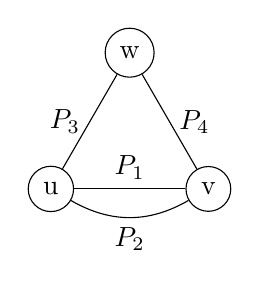
\begin{tikzpicture}
	% Nodes
	\node[circle, draw, fill=white] (u) at (0,0) {u};
	\node[circle, draw, fill=white] (v) at (2,0) {v};
	\node[circle, draw, fill=white] (w) at (1,1.73) {w}; % 1.73 is approximately sqrt(3)
	
	% Edges
	\draw (u) -- (v) node[midway, above] {$P_1$};
	\draw (v) -- (w) node[midway, right] {$P_4$};
	\draw (w) -- (u) node[midway, left] {$P_3$};
	\draw[bend right] (u) to node[midway, below] {$P_2$} (v);
	
\end{tikzpicture}


Por suposicao, o circuito $C_1 = (v,...,u,...,v)$ formado pela concatenacao dos caminhos$P_1$ e $P_2$ tem comprimento impar igual a soma dos comprimentos desses caminhos. Da mesma forma, o circuito $C_2 = (v,w,...,u,...,v)$ formado pela concatenacao dos caminhos $P_2$, $P_3$ e $P_4$ tem comprimento impar igual a soma dos comprimentos desses caminhos. Por fim, o circuito $C_3 = (v,...,u,...,v,w,...,u)$ formado pela concatenacao dos caminhos $P_1$, $P_2$, $P_3$ e $P_4$ tem comprimento impar igual a soma dos comprimentos desses caminhos

\begin{align}
    ||C_1|| &= ||P_1|| + ||P_2|| \\
                &= ||P_1|| + ||P_2|| \\
    ||C_2|| &= ||P_2|| + ||P_3|| + ||P_4|| \\
                &= ||P_2|| + ||P_3||  + 1 \\
  	||C_3|| &= ||P_1|| + ||P_2|| + ||P_3||  + ||P_4|| \\  
  	           &= ||P_1|| + ||P_2|| + ||P_3||  + 1  \\  
\end{align}

Se $P_1$ for ímpar:

\begin{align}
	||C_1|| &= \text{ímpar} + ||P_2|| \\
	&\implies ||P_2|| \text{  é par} \\
	||C_2|| &= ||P_2|| + ||P_3|| + ||P_4|| \\
	&= par + ||P_3||  + 1 \\
	&\implies ||P_3|| \text{   é par} \\
	||C_3|| &= ||P_1|| + ||P_2|| + ||P_3||  +1 \\  
               &= \text{ímpar} + par + par  +1 \\  
               &= \text{ímpar} + \text{ímpar}  \\  
                &\implies 	||C_3|| \text{   é par, o que contradiz a suposicao inicial} \\  
\end{align}


Se $P_1$ for par:

\begin{align}
	||C_1|| &= \text{par} + ||P_2|| \\
	&\implies ||P_2|| \text{  é ímpar} \\
	||C_2|| &= ||P_2|| + ||P_3|| + ||P_4|| \\
	&= \text{ímpar} + ||P_3||  + 1 \\
	&\implies ||P_3|| \text{   é ímpar} \\
	||C_3|| &= ||P_1|| + ||P_2|| + ||P_3||  +1 \\  
	&= \text{par} + \text{ímpar} + \text{ímpar}  +1 \\  
	&= \text{ímpar} + \text{ímpar} + \text{par}  \\  
	&= \text{par} + \text{par}  \\  
	&\implies 	||C_3|| \text{   é par, o que contradiz a suposicao inicial} \\  
\end{align}

Assim, independentemente da paridade de $P_1$, chegamos a uma contradicao. Ou seja, a hipótese de que $G$ nao tem nenhum circuito de comprimento par é falsa.

Portanto, se $G$ é um grafo simples tal que todo vértice tem grau pelo menos $3$, então $G$ contém um circuito de comprimento par.


\clearpage

 \subsection{Exercício 8: Prove por indução em $k$ que o conjunto das arestas de um grafo conexo simples com $2k$ arestas, com $k \geq 1$, pode ser particionado em caminhos de comprimento $2$. A afirmação continuaria válida sem a hipótese de conexidade? Justifique}


 \subsubsection{Caso Base: $k = 1$}
 
 \begin{align}
 	k = 1 &\implies ||E(G)|| = 2k \\
 \end{align}
\begin{align}
	G : 
	\begin{cases} 
		V = [3], \\
	    E = \{ (v_i, v_{i+1}) | i \in \mathbb{Z}, i \leq 2\} \\
	\end{cases}
\end{align}

Uma particao de $E(G)$ que é um caminho de comprimento $2$ é:

\begin{align}
	(X,Y) : 
	\begin{cases} 
		X = (v_1, v_2) \\
		Y = (v_2, v_3) \\
	\end{cases}
\end{align}
 
 
  \subsubsection{Suponhamos que afirmacao e verdadeira para um grafo $G$ com $k = n \geq 2$ vértices} 
  
  Seja $G'$ um grafo conexo tal que $||E(G')|| = 2(n+1) = 2n + 2$.
  
  Como $G$ é conexo e tem $||E(G)|| \geq 1$, pelo menos um de seus vértices $v$ é tal que $d_G(v) \geq 2$.
  
  Sejam $x$ e $y$ vértices de $G'$ adjascentes a $v$. Esses vértices formam um passeio $P = (x,v,y)$ de tamanho $2$.
  
  Se removermos as arestam que formam $P$ de $G'$ restam $2n$ arestas em um grafo $G''$. Assim, $||E(G'')|| = 2n$ e pela hipótese de inducao, $G''$ pode ser particionado em caminhos de comprimento $2$.
  
  Assim, todo grafo simples conexo com  número par de arestas pode ser particionado em caminhos de comprimento $2$. 
  
  Sem a hipótese de conexidade a afirmacao nao continuaria valida, já que é possível definir o seguinte grafo desconexo $F$ que tem um número par de arestas em que nenhum caminho tem comprimento $2$.
 
  \begin{align}
  	F : 
  	\begin{cases} 
  		V = [m] \text{   m é par} \\
  		E = {(u_i, u_j) | u_i, u_j \in V, i , j\text{   sao pares} }\\
  	\end{cases}
  \end{align}
  
  
  \clearpage
  
   \subsection{Exercício 9: Prove que todo grafo simples $G$ pode ser representado como a união de dois grafos disjuntos nas arestas $G_1$ e $G_2$, tais que $G_1$ é acíclico (sem circuitos) e $G_2$ é um grafo par (todos os graus são par).}
      
   
  Para provar que \textit{todo grafo simples $G$ pode ser representado como a união de dois grafos disjuntos nas arestas $G_1$ e $G_2$, tais que $G_1$ é acíclico (sem circuitos) e $G_2$ é um grafo par (todos os graus são par)}, basta:
  
  \begin{itemize}
  	\item Mostrar que se uma aresta de $G$ nao pertence ao subgrafo $G_1$, entao ela pertence as arestas de um subgrafo $G_2$ cujos graus de todos os vertices $d_{G_2}$ sao números pares
  	\item Mostrar que se uma aresta de $G$ nao pertence ao subgrafo $G_2$, entao ela pertence ao conjunto das arestas que nao estao em nenhum ciclo de $G$, isto é, ela pertence a $G_1$
  	\item Nenhuma aresta pode pertencer simultaneamente a $G_1$ e $G_2$
  \end{itemize}
 
 
 \subsubsection{$e \in E(G), e \notin G_1 \implies e  \in G_2 $} 
  
Por definicao, em um circuito cada aresta só pode ser visitada uma única vez. Isso significa que cada vértice $u$ visitado em um circuito a partir de uma aresta $e_i = (u, u_1)$  deve ser adjascente a um vértice $u_2$ pertencente a uma aresta $e_2 = (u,u_2)$ tal que $u_1 \neq u_2$. Em outras palavras, os vizinhos de um vértice $u$ de um circuito podem ser agrupados em pares. Ou seja, o grau dos vértices de um circuito no circuito deve ser par. Se considerarmos os circuitos de $G$ como pertencentes ao subgrafo $G_2$, conclui-se que o grau dos vértices pertencentes a $G_2$  em  $G_2$ é par.


 \subsubsection{$e \in E(G), e \notin G_2\implies e  \in G_1 $} 

Seja uma aresta $(u,v) \in E(G)$ para a qual nao seja possível definir um subgrafo $H \subset G$ tal que $d_{H}(v)$ seja par ou $d_{H}(u)$ seja par. 

Mais especificamente, toda e qualquer trilha $P$ que contenha $(u,v)$ em $G$ é tal que $d_P(u)$ ou $d_P(v)$ sao ímpares. Ou seja, $(u,v) \notin G_2$.

Se $G$ nao possui nenhum circuito que contenha $(u,v)$, conclui-se automaticamente que  $(u,v) \in G_1$.

Suponhamos por absurdo que $G$ possui algum circuito $C$ que contenha $(u,v)$, entao $d_C(u)$ e $d_C(v)$ sao pares, o que se demonstrou anteriormente em relacao a paridade do grau de qualquer vértice pertencente a um circuito no circuito. Isso é uma contradicao, pois $(u,v) \notin G_2$ e, por isso, o grau de pelo menos um deles em \textit{qualquer} trilha de $G$ é ímpar, inclusive em circuitos. Assim, $G$ \textbf{nao} possui nenhum circuito $C$ que contenha $(u,v)$ e, portanto, $(u,v)$ faz parte do conjunto de arestas acíclicas de $G$, $G_1$.


Agora, vamos provar que $ G_1 \cap G_2 = \emptyset $. Seja $k$ o numero de arestas de um grafo $G$. 

\subsubsection{Caso Base: k = 1}

Se $G$ possui apenas uma aresta, $G_2 = \emptyset$ e $G_1$ contem essa única aresta, pois nao é possível construir circuito com uma única aresta. Assim, vale $G_1 \cap G_2 = \emptyset$.


\subsubsection{Assumamos que  vale $G_1 \cap G_2 = \emptyset$ para $k = n$}

Seja $G$ um grafo tal que  $G_1 \cap G_2 = \emptyset$. Seja $e$ uma aresta tal que $e \notin E(G)$. Seja $G'$ o grafo tal que $V(G) \subseteq V(G')$ e $E(G') = E(G) \cup \{e\} $. Ou seja, $G'$  difere de $G$ apenas pela presenca da aresta $e$.

A adicao de $e$ a $G$, resulta, entao, em $G'$ com subconjuntos $G_1'$ e $G_2'$ construidos analogamente a $G_1$ e $G_2$, respectivamente. Tal adicao só pode incorrer em duas consequencias:

\begin{enumerate}[i]
	\item $e$ cria um novo ciclo em $G$. Nesse caso, para definir $G_1'$, basta retirar as $p + 1$ arestas de $G_1$ que formam esse novo ciclo e adicioná-las a $G_2$,  definindo $G_1' = G_1 \setminus \{e_1, ..., e, ..., e_p\}$ e  $G_2' = G_2 \cup \{e_1, ..., e, ..., e_p\}$, usando o que foi demonstrado em $1.5.1$. Nesse caso,  $G_1' \cap G_2' = \emptyset$
	
	\item $e$ nao cria um novo ciclo em $G$. Nesse caso, $e \notin G_2'$ e $G_2' = G_2$. Usando o que foi mostrado em $1.5.2$, entao, $e \in G_1'$. Isso mantem $G_1' \cap G_2' = \emptyset$. 
 \end{enumerate}
 
 Demonstrou-se que a propriedade $G_1' \cap G_2' = \emptyset$  se mantem para $k = n + 1$ e, portanto, $G_1 \cap G_2 = \emptyset$ .
 
 
Assim, todo grafo simples $G$ pode ser representado como a união de dois grafos disjuntos nas arestas $G_1$ e $G_2$, tais que $G_1$ é acíclico (sem circuitos) e $G_2$ é um grafo par (todos os graus são par),  pois   provou-se que $G_1 \cap G_2 = \emptyset$, $e \in E(G), e \notin G_1 \implies e  \in G_2 $ e $e \in E(G), e \notin G_2\implies e  \in G_1 $.

\end{document}
